\chapter{The Standard Model}
\label{chap:sm}

Particle physics endeavours to identify all fundamental units of matter and describe their interactions.
To this end, the Standard Model (SM) of particle physics stands as the most successful theoretical framework in the history of the field.
The SM is a quantum field theory (QFT) that encompasses three of the four fundamental forces of nature: electromagnetic, weak, and strong.
The fourth and final force, gravity, is not included in the SM\footnote{Gravity is $10^{37}$ times weaker than the weak nuclear force, and thus is negligible at the energy scales probed by particle accelerators, but can be incorporated to the theory through a coupling to a curved space-time.}.
The development of the SM was an iterative and collaborative effort that took much of the 20th century, during a time which saw great strides in the available technology, experimental techniques, and theory.
No experimental evidence has been found to contradict the SM predictions, much to the chagrin of many physicists who are eager to find the next breakthrough.

\section{Particle Content}

The SM describes all matter and forces in the universe using only 17 fundamental particles.
These particles are categorized by their spin.
Fermions have spin-$\sfrac{1}{2}$ (in units of $\hbar$), and obey Fermi-Dirac statistics.
Bosons have integer spin and obey Bose-Einstein statistics.
Fermions make up all physical matter in the universe, while spin-1 bosons mediate the forces between them.

There are 12 fermions in the SM, divided into two categories: leptons and quarks.
Fermions come in three generations, each containing a charged lepton, a neutral lepton (neutrino), an up-type quark, and a down-type quark.
Each subsequent generation contains particles with increased mass but identical quantum numbers to the preceding one.
Heavier generations are therefore unstable and decay into the lighter generations.
The exceptions to this rule are the neutrinos, which do not decay, but oscillate between the three generations~\cite{NeutrinoOsc}.
% The first generation contains the lightest particles; the electron, electron neutrino, up quark, and down quark.
% The second generation contains the muon, muon neutrino, charm quark, and strange quark.
% Finally, the third generation contains the tau, tau neutrino, top quark, and bottom quark.
Each fermion has an associated antiparticle with the same mass and spin but an opposite charge and baryon number.
Fermions also have distinct left- and right-handed chiral states which are treated differently in the SM\@.
A list of the fermions and their properties can be found in Table~\ref{tab:fermions}.

\begin{table}[h]
	\centering
	\caption{Fermions (spin-$\sfrac{1}{2}$ particles) of the Standard Model and their properties~\cite{ParticleDataGroup}. Not shown are the antiparticles, which have opposite charge and baryon number, but are otherwise identical.}
	\begin{adjustbox}{max width=\textwidth}
		\label{tab:fermions}
		\renewcommand{\arraystretch}{1.5}
		\begin{tabular}{c|cccc|cccc}
			\toprule
			\hline
			                        & \multicolumn{4}{c}{Leptons} & \multicolumn{4}{|c}{Quarks}                                                                                                   \\
			\hline
			Generation              & Flavour                     & Symbol                      & Mass $[\MeV]$          & Charge $[e]$ & Flavour & Symbol & Mass $[\MeV]$      & Charge $[e]$    \\
			\hline
			\multirow{2}{*}{First}  & electron                    & $e$                         & 0.5110                 & -1           & up      & $u$    & 2.16               & $+\sfrac{2}{3}$ \\
			                        & $e$-neutrino                & $\nu_e$                     & $< 0.8 \times 10^{-6}$ & 0            & down    & $d$    & 4.70               & $-\sfrac{1}{3}$ \\
			\hline
			\multirow{2}{*}{Second} & muon                        & $\mu$                       & 105.7                  & -1           & charm   & $c$    & $1.27 \times 10^3$ & $+\sfrac{2}{3}$ \\
			                        & $\mu$-neutrino              & $\nu_\mu$                   & $< 0.19$               & 0            & strange & $s$    & 93.5               & $-\sfrac{1}{3}$ \\
			\hline
			\multirow{2}{*}{Third}  & tau                         & $\tau$                      & 1777                   & -1           & top     & $t$    & $173 \times 10^3$  & $+\sfrac{2}{3}$ \\
			                        & $\tau$-neutrino             & $\nu_\tau$                  & $< 18.2$               & 0            & bottom  & $b$    & $4.18 \times 10^3$ & $-\sfrac{1}{3}$ \\
			\hline
		\end{tabular}
	\end{adjustbox}
\end{table}

Forces between fermions in a QFT manifest via the exchange of spin-1 particles called vector- or gauge-bosons.
For a particle to interact with a given vector-boson, it must carry the corresponding charge.
The massless photon mediates the electromagnetic force and the charge is the familiar electric charge $Q$.
All fermions other than the neutrinos carry electromagnetic charge.
Interactions via the weak force come in two forms, charged and neutral, and they are mediated by the $W^\pm$ and $Z$ bosons respectively.
The charges of the weak force are weak isospin $I$ and hypercharge $Y$.
All fermions carry hypercharge but only left-handed fermions and right-handed antifermions carry weak isospin.
Interactions via the charged weak bosons are the only interaction which allows a change in the flavour of a fermion, e.g.\ a down-type quark can change into an up-type quark by emitting a $W^-$ boson.
Unlike the other forces in the SM, the bosons of the weak force have non-zero mass, resulting in a short range of interaction.
The strong force is mediated by the massless gluon and is carried by the colour charge.
Out of the fermions, only the quarks carry colour charge, which has three possible values labelled red, green, and blue.
Anti-quarks carry an anti-colour charge, which are anti-red, anti-green, and anti-blue.
Gluons also carry the colour charge; an eightfold combination of one colour and one anti-colour.

The last particle in the SM is the Higgs boson, a scalar particle with spin-0 which couples to all massive particles.
A summary of the bosons and their properties can be found in~\Cref{tab:bosons}.

\begin{table}[h]
	\centering
	\caption{Bosons (interger spin particles) of the Standard Model and their properties~\cite{ParticleDataGroup}.
		The spin $J$ and parity $P$ of each particle are denoted by $J^P$. The strengths of the forces associated with each boson are given relative to the strong force at a distance of 1 \unit{\femto\metre}.}
	\begin{adjustbox}{max width=\textwidth}
		\label{tab:bosons}
		\renewcommand{\arraystretch}{1.5}
		\begin{tabular}{lclccccc}
			\toprule
			\hline
			Force                   & Strength                   & Boson                & Symbol   & Spin & Charge $[e]$ & Mass $[\GeV]$ & $J^P$ \\
			\hline
			Strong                  & $1$                        & Gluon                & $g$      & 1    & 0            & 0             & $1^-$ \\
			Electromagnetic         & $1^{-3}$                   & Photon               & $\gamma$ & 1    & 0            & 0             & $1^-$ \\
			\multirow{2}{*}{Weak}   & \multirow{2}{*}{$10^{-8}$} & Weak boson (charged) & $W^\pm$  & 1    & $\pm 1$      & $80.37$       & $1^-$ \\
			                        &                            & Weak boson (neutral) & $Z$      & 1    & 0            & $91.19$       & $1^-$ \\
			\hline
			\multicolumn{2}{c}{N/A} & Higgs boson                & $H$                  & 0        & 0    & $125.2$      & $0^+$                 \\
			\hline
		\end{tabular}
	\end{adjustbox}
\end{table}

\section{The Gauge Principle}
\label{sec:gauge_principle}

Most of the breakthroughs in theoretical physics have been driven by the search for symmetries in nature.
Noether's theorem famously established that continuous symmetries imply conserved currents~\cite{Noether1918}.
The principle of least action states that the dynamics of a system are determined by the path through spacetime that minimizes the action specified by a Lagrangian density $\mathcal{L}$.
The Lagrangian of the SM is symmetrical under the global Poincaré group, $\text{SL}(2, \mathbb{C})$, which encompasses the symmetries of special relativity.
Under Noether's theorem, this directly leads to the conservation of energy and momentum.
Herman Weyl, a colleague of Noether, extended this to the principle of gauge theory; a field theory where the dynamics of a system could be determined by requiring invariance under local (non-global), smooth transformations~\cite{GaugeSym}.
Weyl's \textit{gauge principle} showed that if a free field Lagrangian was required to be invariant under local transformations belonging to an Abelian group, then the extra interaction terms would arise naturally.
Chen Yang and Robert Mills generalized this theory to non-Abelian groups~\cite{YangMills}.

\subsection{Free Field Lagrangians}

The starting point of the gauge principle is the Lagrangian density of free fields.
In a QFT, all fundamental objects are described by quantum fields which are themselves functions of spacetime $x = (t, \vec{x})$.
Observed particles are localized excitations of these fields.
The free field Lagrangian densities describe the propagation of non-interacting objects through spacetime and their forms depend on the spin of the particle.

Spin-0 particles are excitations of a scalar field $\phi(x)$ such that they obey the Klein-Gordon equation~\cite{Klein1926} and the corresponding Lagrangian density,
\begin{equation}
	\label{eq:scalar_lagrangian}
	\mathcal{L}_\text{S} = \frac{1}{2} \partial_\mu \phi \partial^\mu \phi - \frac{1}{2} m_S^2 \phi^2,
\end{equation}
where $m_S$ is the mass of the particle, $\mu$ runs over the four dimensions of spacetime, and the Einstein summation convention is used.
Spin-$\sfrac{1}{2}$ particles are described by the 4-component Dirac spinor $\psi(x)$ and the equations of motion are described by the Dirac Lagrangian density~\cite{Dirac1928},
\begin{equation}
	\label{eq:dirac_lagrangian}
	\mathcal{L}_\text{Dirac} = \bar{\psi} (i \gamma^\mu \partial_\mu - m) \psi.
\end{equation}
Here, $\gamma^\mu(\mu=0,1,2,3)$ are the contravariant Dirac matrices\footnote{The Dirac matrices are defined by the anti-commutation relations$\{ \gamma^\mu, \gamma^\nu \} = 2 g^{\mu\nu}$, where $g^{\mu\nu}$ is the Minkowski metric.}, $\bar{\psi} = \psi^\dagger \gamma^0$ is the Dirac adjoint, and $m$ is the mass of the fermion.
Finally, free spin-1 vector fields $A_\mu$ with mass $m_A$ are described by the Proca Lagrangian,
\begin{equation}
	\label{eq:proca_lagrangian}
	\mathcal{L}_\text{Proca} = -\frac{1}{4} F_{\mu\nu} F^{\mu\nu} + \frac{1}{2} m_A^2 A_\mu^a A^{\mu},
\end{equation}
where $F_{\mu\nu}^a$ is the field strength tensor.

\subsection{Local Gauge Invariance}

In a gauge theory, $\mathcal{L}$ is assumed to be invariant under a set of transformations which form a Lie group $G$.
Any element of a Lie group $g \in G$ can be written as a product of exponentials of generators $g = \exp(i \theta_a T^a)$, where $\theta_a$ are the phase parameters and $T^a$ are the group generators (members of the corresponding Lie algebra).
Local gauge invariance is expressed as phase parameters which depend on spacetime $\theta_a(x)$ and $\mathcal{L}$ is therefore required to be invariant under the transformation,
\begin{equation}
	\label{eq:local_gauge_invariance}
	\psi \rightarrow \exp\left(i \theta_a(x) T^a\right) \psi.
\end{equation}
Using fermions as an example, it is clear that $L_\text{Dirac}$ is not invariant under local phase transformations.
To remedy this, the covariant derivative $D_\mu$ is introduced,
\begin{equation}
	\label{eq:covariant_derivative}
	D_\mu = \partial_\mu - i g T^a A_\mu^a,
\end{equation}
where $A_\mu^a$ represents a spin-1 vector field for each generator and $g$ is a scalar called the coupling constant.
The field itself is required to transform as,
\begin{equation}
	\label{eq:gauge_transformation}
	A_\mu^a \rightarrow A_\mu^a - g^{-1} \partial_\mu \theta^a - f^{abc} \theta^b A_\mu^c,
\end{equation}
where $f^{abc}$ are the structure constants of $G$ given by the relation,
\begin{equation}
	\label{eq:structure_constants}
	[T^a, T^b] = i f^{abc} T^c.
\end{equation}
The term on the left denotes the commutator Lie bracket $[A, B] = AB - BA$.
In an Abelian group, the structure constants are all trivially zero.
Inserting the covariant derivative into the Dirac Lagrangian density yields,
\begin{align}
	\label{eq:dirac_lagrangian_gauge}
	\mathcal{L_D} & = \bar \psi (i \gamma^\mu D_\mu - m) \psi                                                                                                                                       \\
	              & = \underbrace{\bar \psi (i \gamma^\mu \partial_\mu - m) \psi}_\text{free spinor} \quad + \quad \underbrace{g \bar \psi \gamma^\mu A_\mu^a \psi}_\text{\shortstack{spinor-vector \\interaction}}.
\end{align}
$\mathcal{L}_D$ is the modified Dirac Lagrangian which no longer describes a free fermion field $\psi$ but one that interacts with a vector field $A_\mu^a$ and the strength of the interaction is proportional to the coupling constant $g$.

The existence of $A_\mu^a$ also means that it should contribute to the Lagrangian density of the system via \Cref{eq:proca_lagrangian}.
The field strength tensor (generalized to non-Abelian groups) is described by,
\begin{equation}
	\label{eq:field_strength_tensor}
	F_{\mu\nu}^a = \partial_\mu A_\nu^a - \partial_\nu A_\mu^a - g f^{abc} A_\mu^b A_\nu^c
\end{equation}
allowing the construction of the full Lagrangian density for the vector boson field,
\begin{align}
	\label{eq:boson}
	\mathcal{L}_\text{Proca} =
	 & \vphantom{\cancelto{0}{m_A^2}} -\frac{1}{4}(\partial_\mu A_\nu^a - \partial_\nu A_\mu^a) (\partial^\mu A^{a,\nu} - \partial^\nu A^{a,\mu}) &  & \leftarrow \text{dynamics}            \\
	 & \vphantom{\cancelto{0}{m_A^2}} + \frac{1}{2} g f^{abc} (\partial_\mu A_\nu^a - \partial_\nu A_\mu^a) A^{b\mu} A^{c\nu}                     &  & \leftarrow \text{triple interaction}  \\
	 & \vphantom{\cancelto{0}{m_A^2}} - \frac{1}{2} g^2 f^{abc} f^{ade} A_\mu^b A_\nu^c A^{d\mu} A^{e\nu}                                         &  & \leftarrow \text{quartic interaction} \\
	 & + \frac{1}{2} \cancelto{0}{m_A^2} A_\mu^a A^{a,\mu}                                                                                        &  & \leftarrow \text{mass term}.
\end{align}
Note is that the mass term for the vector boson has been crossed out.
This is because the quadratic $A_\mu^a A^{a,\mu}$ is not invariant under the transformation of \Cref{eq:gauge_transformation}, leading to the conclusion that either the vector boson is massless or that the symmetry is broken.
On the other hand, the terms derived from the field strength tensor $F_{\mu\nu}^a F^{a,\mu\nu}$ are invariant under the local gauge transformation.
In the non-Abelian case (non-zero structure constants), the Lagrangian includes additional interaction terms between the $A_\mu^a$ field and itself called triple and quartic self-couplings.

Therefore, the necessity for local gauge invariance of a theory of fermions suggests the presence of new massless gauge fields characterized by specific gauge transformation properties.
Furthermore, each of the group generators correspond to a hermitian operator, related to the charge of the interaction.
The full Lagrangian for the system $\mathcal{L} = \mathcal{L}_D + \mathcal{L}_\text{Proca}$ contains terms for the free fermion field, interactions between fermion field and the gauge fields, and self-interactions terms of the gauge fields if the group is non-Abelian.

\section{Symmetries of the Standard Model}
\label{sec:symmetries_of_sm}

The Lie group of local gauge transformations observed by the SM Lagrangian can be expressed as the product of three simple groups,
\begin{equation}
	\label{eq:sm_group}
	\text{SU}(3)_C \times \text{SU}(2)_L \times \text{U}(1)_Y.
\end{equation}
Here the subscript $C$ denotes the colour charge and, $L$ refers to left-handed fermions only, and $Y$ is the hypercharge.
Adherence to $\text{SU}(3)_C$ gives rise to interactions via the strong force, which is outlined in \Cref{sec:qcd}.
The $\text{SU}(2)_L \times \text{U}(1)_Y$ group corresponds to the unified forces of electromagnetism and the weak force, which is described in \Cref{sec:electroweak}.

The full Lagrangian of the SM is given by,
\begin{equation}
	\label{eq:sm_lagrangian}
	\mathcal{L}_\text{SM} =
	\overbrace{
		\vphantom{\frac{1}{4}}
		i \bar \psi \gamma^\mu D_\mu \psi
	}^{\mathcal{L}_{D}^{m=0}
	}
	\overbrace{
		-\frac{1}{4} F_{\mu\nu} F^{\mu\nu}
	}^{\mathcal{L}_{Proca}^{m=0}
	}
	\overbrace{
		+
		\underbrace{
			\vphantom{\frac{1}{4}}
			(y_{ij} \bar \psi_i \phi \psi_j
			+ \text{h.c.})
		}_{\text{Yukawa couplings}}
		+ |D_\mu \phi|^2
		- V(\phi)
	}^{\text{Higgs sector}},
\end{equation}
The first term $\mathcal{L}_D^{m=0}$ refers to fermions and their interactions with the gauge-bosons.
The second term $\mathcal{L}_{Proca}^{m=0}$ refers to gauge-boson dynamics and their self couplings.
Note that for both of these terms the mass of the fields is set to zero.
This is because mass in the SM are generated through interaction with the Higgs field $\phi$.
Fermion mass is described by the Yukawa interaction, where $y_{ij}$ are the Yukawa coupling constants and h.c.\ denotes the Hermitian conjugate.
The last two terms describe the Higgs interaction with the massive vector bosons and the Higgs potential, respectively.
The Higgs mechanism described in \Cref{sec:higgs}.

In the SM there are also three important discrete symmetries.
Namely, charge conjugation $\mathcal{C}$, parity inversion $\mathcal{P}$, and time reversal $\mathcal{T}$.
Each of these symmetries were once believed to be obeyed by all physical processes.
However, $\mathcal{P}$ violation was first observed in 1956~\cite{Wu1957} and the combined symmetry $\mathcal{CP}$ was shown to be violated in 1964~\cite{CPViolation}.
In the SM it is now known that the weak force can violate any combination of $\mathcal{C}$, $\mathcal{P}$, and $\mathcal{T}$, but not all simultaneously.
In fact, the combined symmetry $\mathcal{CPT}$ holds for all Lorentz invariant QFTs and is therefore beleived to be obeyed by all physical processes.


\subsection{U(1) \texorpdfstring{$\rightarrow$}{-} Quantum Electrodynamics}

The discovery of the electron in 1897 marked the first major breakthrough in particle physics~\cite{ThomsonElectron}.
In 1926, Oskar Klein and Walter Gordon attempted to merge quantum mechanics and special relativity to describe a relativistic electron~\cite{Klein1926,Gordon1926}.
Two years later, Paul Dirac incorporated electron spin into the theory, introducing the concept of antiparticles~\cite{Dirac1928}.
Soon after, Dirac's predicted positron was observed~\cite{PositiveElectron}, marking the first time a particle was discovered after being predicted theoretically.
Fermi's theory of $\beta$-decay~\cite{Fermi1934} showed that it was possible to describe annihilation and creation of particles using QFT\@, solidifying it as the correct framework for particle physics.
In all QFTs, the scattering amplitudes are calculated via perturbative expansion of interaction terms in the Lagrangian using a Dyson series~\cite{AlexQED4}.
This expansion lead to divergent and non-physical results for basic quantities such as the self-energy of the electron.
More than a decade later, this crisis was resolved by the method of renormalization~\cite{Renorm1,Renorm2,Renorm3,Renorm4,Renorm5,Renorm6,Renorm7,Renorm8,Renorm9,Renorm10,Renorm11,Renorm12}, which absorbs these infinities at the cost of introducing a dependence on the energy scale of the interaction for the effective coupling constants.
With this new technique, quantum electrodynamics (QED)~\cite{AlexQED1,AlexQED2,AlexQED3} was fully established as a complete description of the electromagnetic force.

All gauge theories start with the assumption of a local symmetry and the simplest of these is $\text{U}(1)$.
For fermion fields this is expressed as $\psi \rightarrow \exp{\left(i Q \chi(x)\right)} \psi$, for some arbitrary scalar $\chi(x)$ and coupling strength (electric charge) $Q$.
Assuming this symmetry is respected by the Dirac Lagrangian, then following the procedure in \Cref{eq:gauge_transformation}, a new vector field $A_\mu$ is introduced transforming as,
\begin{equation}
	\label{eq:photon_transformation}
	A_\mu \rightarrow A_\mu - \partial_\mu \chi.
\end{equation}
As $\text{U}(1)$ is Abelian, the structure constants disappear and the vector field does not self-interact.
This results in the QED Lagrangian density,
\begin{align}
	\mathcal{L}_\text{QED} & = \overbrace{-\frac{1}{4} F_{\mu\nu} F^{\mu\nu}}^{\text{free photon}}
	+ \overbrace{\vphantom{\frac{1}{1}}\bar \psi (i \gamma^\mu \partial_\mu - m) \psi}^{\text{free fermion}}
	+ \overbrace{\vphantom{\frac{1}{1}}Q \bar \psi \gamma^\mu A_\mu \psi}^{\text{interaction}}               \\
	                       & = -\frac{1}{4} F_{\mu\nu} F^{\mu\nu} + \bar \psi (i \gamma^\mu D_\mu - m) \psi.
	\label{eq:qed_lagrangian}
\end{align}
Note that the interaction term is absorbed into the covariant derivative in \Cref{eq:qed_lagrangian}.

By the simple requirement that physics is invariant under a local $\text{U}(1)$ transformation, an interaction arises between the fermion field and a massless spin-1 field, where the strength of these interactions is proportional to $Q$.
These two features are now known to be the photon field and the electric charge.
In the SM, $\mathcal{L}_\text{QED}$ is absorbed into the electroweak Lagrangian density, described in \Cref{sec:electroweak}.

\subsection{\texorpdfstring{$\text{SU(3)}_C\rightarrow$}{SU(3)-} Quantum Chromodynamics}
\label{sec:qcd}

Starting with the discovery of the pion in 1947~\cite{DiscoveryPimeson} a veritable explosion of new hadrons were detected.
This was largely due to the development of the first particle accelerators~\cite{ProductionHighSpeed} which allowed for the study of controlled high-energy collisions outside cosmic rays.
This period of discovery lasted until the mid 1960s and a description of the expanding list of particles was needed.
Initial attempts involved the introduction of new quantum numbers such as strangeness~\cite{Strange2, Strange3} and isospin~\cite{StrongIso1, StrongIso2, StrongIso3,StrongIso4}.
This \textit{particle zoo} was eventually tamed by the theory of quarks in 1964 by Gell-Mann and Zweig~\cite{GellMan1964,Zweig1964}.
Each of these new particles could be understood as a bound state of multiple quarks called hadrons.
Two- and three-quark states correspond to mesons and baryons, respectively.
Quarks were experimentally confirmed by deep inelastic collision experiments in 1969~\cite{Quark1, Quark2}.
The theory of quarks and their interactions via the strong force was formulated as a renormalizable QFT called quantum chromodynamics (QCD) in the early 1970s~\cite{QCD1,QCD2,QCD3}.

The $\text{SU}(3)_C$ symmetry group is an eight-dimensional group often expressed by all $3 \times 3$ unitary matrices with determinant 1.
The eight generators of the group are typically expressed as using the Gell-Mann matrices $\lambda^a$~\cite{GellManMatrix},
\begin{equation}
	\label{eq:su3_generators}
	T^a = \frac{\lambda^a}{2}, \quad a = 1, \ldots, 8.
\end{equation}
The phase parameters $\theta^a(x)$ are therefore also eight separate functions of spacetime.
The group is non-Abelian, making it a Yang-Mills theory, and the non-zero structure constants are given by,
\begin{equation}
	\label{eq:qcd_sc}
	\begin{array}{ccc}
		f_{123} = 1 ,                                                            & \hspace{\stretch{1}}
		f_{147} = f_{516} = f_{246} = f_{257} = f_{345} = f_{637} = \frac{1}{2}, & \hspace{\stretch{1}}
		f_{458} = f_{678} = -\frac{1}{2}.
	\end{array}
\end{equation}
The eight dimensional group corresponds to eight massless vector fields $G_\mu^a$ which are the gluons, and together with the strong coupling constant $g_s$ they yield the QCD covariant derivative,
\begin{equation}
	\label{eq:qcd_covariant_derivative}
	D_\mu = \partial_\mu - i g_s T^a G_\mu^a.
\end{equation}
The transformation properties of the gluon fields are given by \Cref{eq:gauge_transformation}, and the field strength tensor is given by \Cref{eq:field_strength_tensor}.
To express this new color charge, the fermion spinor $\psi$ acquires three new degrees of freedom represented by the quark field $q_i\:(i = 1, 2, 3)$.
The QCD Lagrangian density,
\begin{equation}
	\label{eq:qcd_lagrangian}
	\mathcal{L}_\text{QCD} = -\frac{1}{4} G_{\mu\nu}^a G^{a,\mu\nu} + \bar q_i (i \gamma^\mu D_\mu - m) q_i.
\end{equation}

For the electromagnetic and weak forces the coupling strength increases with the momentum transfer of the interaction, but this dependence is minor.
For the strong force the coupling constant becomes significantly weaker as the energy scale increases and the length scale decreases.
This is a phenomenon known as asymptotic freedom~\cite{PriceAsymptoticFreedom} and is shown in \Cref{fig:asymptotic_freedom}.
At the high energies of collider experiments ($ > 100 \GeV$), the quarks, even though bound in hadrons, behave as free particles.
Conversely, at low energies the coupling constant becomes close to unity.
At these scales divergences are induced and the theory can't be treated perturbatively.

\begin{figure}[h]
	\centering
	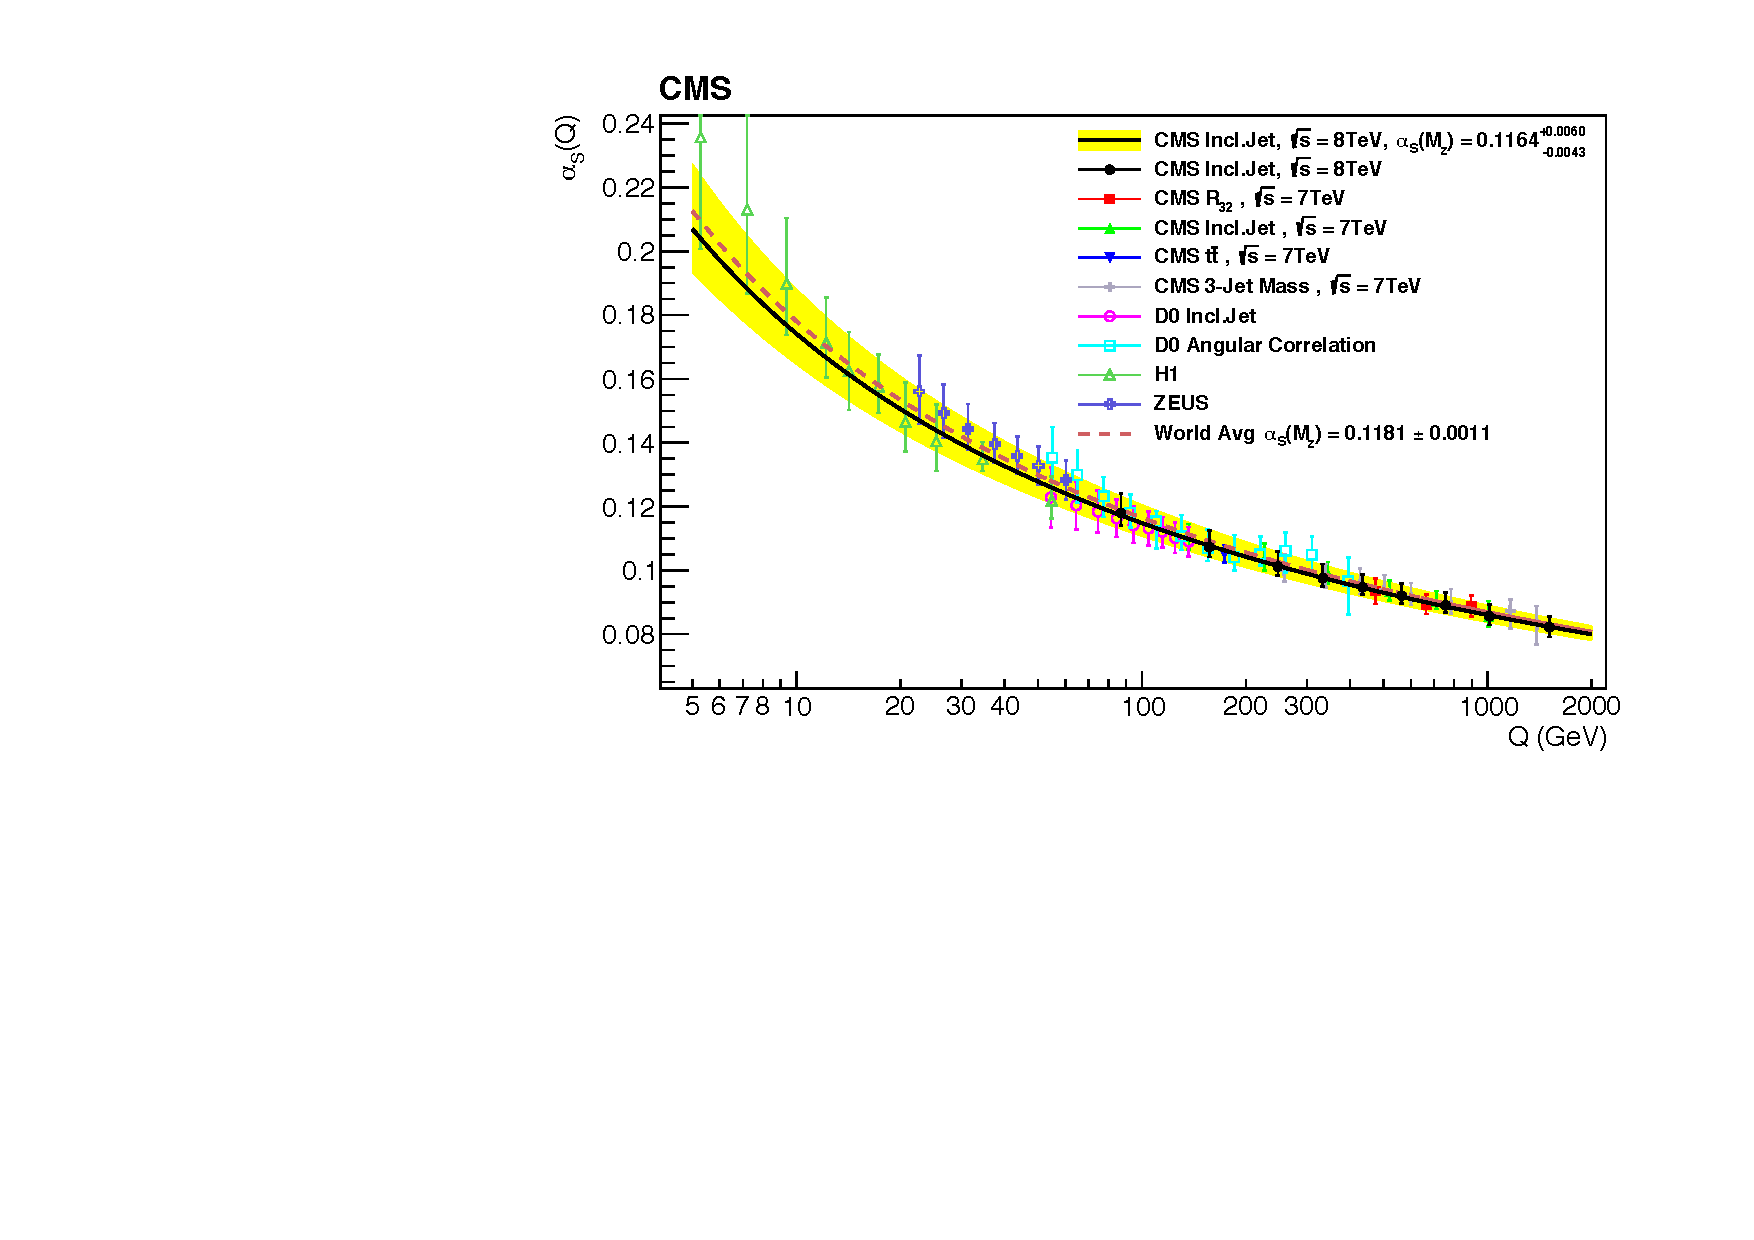
\includegraphics[width=0.7\textwidth]{Figures/standard_model/running}
	\caption{The running of the strong coupling constant $\alpha_s = \sfrac{g_s^2}{4\pi}$ as a function of the energy scale $Q$ as measured by experiments at the LHC, Tevatron, and HERA~\cite{CMSRunning}.}
	\label{fig:asymptotic_freedom}
\end{figure}

An observed effect of QCD is \textit{colour confinement}, where quarks and gluons are never observed isolated, but always bound together in colour-neutral ($\text{SU}(3)$ invariant) states called hadrons.
This is illustrated by the qualitative picture in \Cref{fig:confinement}.
For an electromagnetic interaction, \Cref{fig:confinement_b}, the field is diluted over space.
However, for a strong interaction, \Cref{fig:confinement_c}, the exchanged gluons themselves interact, \Cref{fig:confinement_a}, effectively squeezing the colour field between the quarks into a \textit{color flux tube} or a \textit{color string}.
These strings have a constant energy density so two free quarks on opposite sides of the universe would theoretically result in a string of near-infinite energy.
As the theory is non-perturbative, there is no analytical description for confinement.
A consequence of confinement is hadronisation, the process by which high energy coloured particles form particle jets, which is described in \Cref{sec:jets}.

\begin{figure}[h]
	\centering
	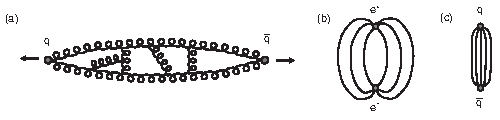
\includegraphics[width=0.8\textwidth]{Figures/standard_model/confinement.pdf}
	\begin{subfigure}{0pt}\phantomcaption{}\label{fig:confinement_a}\end{subfigure}
	\begin{subfigure}{0pt}\phantomcaption{}\label{fig:confinement_b}\end{subfigure}
	\begin{subfigure}{0pt}\phantomcaption{}\label{fig:confinement_c}\end{subfigure}
	\caption{Qualitative picture of the formation of colour strings due to interaction between the exchanged gluons from two quarks \cite{ModernParticlePhysics}.}.
	\label{fig:confinement}
\end{figure}

\subsection{\texorpdfstring{$\text{SU}(2)_L \times \text{U}(1)_Y \rightarrow$}{SU(2)xSU(1)-} Electroweak Theory}
\label{sec:electroweak}

In 1934 Fermi's description of $\beta$ decay~\cite{Fermi1934} hypothesized the existence of the weak nuclear force and allowed for the creation and annihilation of particles.
Around three decades later the Glashow-Weinberg-Salam model (GSW)~\cite{Glashow1961, Weinberg1967,Salam1964} was developed to unify the electromagnetic and weak forces using the comined $\text{SU}(2)_L \times \text{U}(1)_Y$.
As with all gauge theories, this introduces four gauge fields corresponding to each generator of the group.
\begin{align}
	\text{SU}(2)_L & \rightarrow W_\mu^a(a = 1, 2, 3) \\
	\text{U}(1)_Y  & \rightarrow B_\mu
\end{align}
The $\text{SU}(2)_L$ group is non-Abelian making this a Yang-Mills theory, and the structure constants are given by $f^{abc} = \epsilon^{abc}$, where $\epsilon^{abc}$ is the Levi-Civita symbol.
The generators of the group are the based on the three Pauli spin matrices $\sigma^i$.
\begin{equation}
	\label{eq:su2_generators}
	T^a \equiv I^a = \frac{\sigma^a}{2} \\
\end{equation}
\begin{equation}
	\sigma^1 = \begin{pmatrix} 0 & 1 \\ 1 & 0 \end{pmatrix},
	\quad \sigma^2 = \begin{pmatrix} 0 & -i \\ i & 0 \end{pmatrix},
	\quad \sigma^3 = \begin{pmatrix} 1 & 0 \\ 0 & -1 \end{pmatrix}.
	\label{eq:pauli_matrices}
\end{equation}
The strength tensors are given by
\begin{align}
	\label{eq:ew_field_strength_tensors}
	W_{\mu\nu}^a & = \partial_\mu W_\nu^a - \partial_\nu W_\mu^a - g \epsilon^{abc} W_\mu^b W_\nu^c, \\
	B_{\mu\nu}   & = \partial_\mu B_\nu - \partial_\nu B_\mu.
\end{align}
It is useful to split the fermion fields into left- and right-handed components using chiral the projection operators $P_{L/R} = \sfrac{1}{2} (1 \mp \gamma^5)$, where $\gamma^5 = i \gamma^0 \gamma^1 \gamma^2 \gamma^3$.
Experimentally, the charged weak current has proved to maximally violate $\mathcal{P}$ symmetry.
This means that the interaction term must follow a V-A (vector-axial) coupling type which can be shown to be equivalent to a standard coupling to left-handed fermions only:
\begin{equation}
	\label{eq:v-a_coupling}
	\mathcal{L}_\text{V-A}
	= \frac{1}{2} \bar \psi \gamma^\mu (1 - \gamma^5) \psi W_\mu
	= \bar \psi \gamma^\mu P_L \psi W_\mu
	= \bar \psi P_R \gamma^\mu P_L \psi W_\mu
	= \bar \psi_L \gamma^\mu \psi_L W_\mu.
\end{equation}
Therefore, only left-handed fermions (and right-handed antifermions) carry non-zero weak isospin.
The covariant derivative is given by,
\begin{equation}
	\label{eq:ew_covariant_derivative}
	D_\mu = \partial_\mu - i g_W \frac{\sigma_a}{2} W_\mu^a - i g_Y \frac{Y}{2} B_\mu,
\end{equation}
where $g_W$ and $g_Y$ are the weak and hypercharge coupling constants respectively.
The Lagrangian for electroweak theory is,
\begin{align}
	\begin{split}
		\label{eq:ew_lagrangian}
		\mathcal{L}_\text{EW} = & - \bar{\psi}_L \left( \gamma^\mu g_W \frac{1}{2} \sigma^a W^a_\mu + \gamma^\mu g_Y \frac{Y}{2} B_\mu \right) \psi_L - \bar{\psi}_R \left( \gamma^\mu g_Y \frac{Y}{2} B_\mu \right) \psi_R \\
		                        & - \frac{1}{4} W_{\mu\nu}^a W^{a,\mu\nu} - \frac{1}{4} B_{\mu\nu} B^{\mu\nu}.
	\end{split}
\end{align}
As a Yang-Mills theory, the gauge fields $W_\mu^a$ interact in quadratic and triple self-couplings.

The $2 \times 2$ Pauli matrices require two new components to the fermion wave function which are described as weak isospin doubles.
The left-handed fermions (and right-handed antifermions)
are placed in doublets which differ by a unit of charge.
Up-type quarks and neutrinos have a weak isospin of $\sfrac{1}{2}$, while down-type quarks and charged leptons have a weak isospin of $-\sfrac{1}{2}$.
The corresponding weak eigenstate doublets are given by,
\begin{equation}
	\label{eq:weak_isospin}
	\begin{pmatrix} \nu_e \\ e \end{pmatrix}_L,
	\begin{pmatrix} \nu_\mu \\ \mu \end{pmatrix}_L,
	\begin{pmatrix} \nu_\tau \\ \tau \end{pmatrix}_L,
	\begin{pmatrix} u \\ d' \end{pmatrix}_L,
	\begin{pmatrix} c \\ s' \end{pmatrix}_L,
	\begin{pmatrix} t \\ b' \end{pmatrix}_L.
\end{equation}
The right-handed fermions (and left-handed antifermions) do not carry isospin and are placed in singlets.
The effect of the charged weak interaction is therefore to rotate these doublets, effectively changing the flavour of the fermion\footnote{Since there is no other force through which the neutrinos can interact, there are no right-handed neutrinos in the SM.}.

The isospin doublets are described with respect to the weak eigenstates, which do not correspond to the observable mass eigenstates.
The down-type quarks by convention mix between the weak eigenstates ($d', s', b'$) and the mass eigenstates ($d, s, b$) through the CKM matrix~\cite{cabibbo1963},
\begin{equation}
	\label{eq:ckm_matrix}
	\begin{pmatrix} d' \\ s' \\ b' \end{pmatrix} =
	\begin{pmatrix} V_{ud} & V_{us} & V_{ub} \\ V_{cd} & V_{cs} & V_{cb} \\ V_{td} & V_{ts} & V_{tb} \end{pmatrix} \begin{pmatrix} d \\ s \\ b \end{pmatrix} =
	\begin{pmatrix} 0.974 & 0.224 & 0.004 \\ 0.221 & 0.975 & 0.041 \\ 0.009 & 0.042 & 1.014 \end{pmatrix} \begin{pmatrix} d \\ s \\ b \end{pmatrix},
\end{equation}
where the numerical values of the elements are determined experimentally~\cite{ParticleDataGroup}\footnote{The non-unitary nature of experimental values of the CKM matrix is in tension with the SM by 2.2$\sigma$}.
For the leptons, the mixing is described with respect to the neutrinos and the PMNS matrix~\cite{PMNSMatrix}.
These matrices provide explanations for the observed neutrino oscillations and the CP violation of the weak sector.

\section{Electroweak Symmetry Breaking}
\label{sec:higgs}

In 1964, the mechanism for which spontaneous symmetry breaking could lead to massive gauge-bosons was developed independently by Robert Brout and François Englert, and Peter Higgs.
This was incorporated into the electroweak theory by Steven Weinberg and Abdus Salam, and the theory was shown to be renormalizable.
Experimental evidence for the electroweak theory first came in 1983 with the discovery of the W and Z bosons at CERN\@.
Arguably the last major breakthrough in the field of particle physics was the discovery of the Higgs boson in 2012 by the ATLAS and CMS collaborations.
Over 100 years after the discovery of the electron.

GSW theory predicts 4 gauge fields $W^a_\mu$ and $B_\mu$ which do not correspond to the physical $W^\pm$, $Z$, and $\gamma$ bosons.
As a requirement of gauge invariance these fields are deemed to be massless, which is also in contradiction with the observed massive $W^\pm$ and $Z$ bosons.
These discrepancies are resolved by the Brout-Englert-Higgs mechanism~\cite{Higgs1, Higgs2, Higgs3} (referred to hereafter as the Higgs mechanism), and the spontaneous symmetry breaking of the electroweak symmetry group (EWSB).
Spontaneous symmetry breaking is a phenomenon where the ground state of a system does not exhibit the same symmetries of the Lagrangian.

Consider a new scalar field given by a complex doublet,
\begin{equation}
	\phi = \begin{pmatrix} \phi^+ \\ \phi^0 \end{pmatrix} = \frac{1}{\sqrt{2}} \begin{pmatrix} \phi_1 + i \phi_2 \\ \phi_3 + i \phi_4 \end{pmatrix},
\end{equation}
embedded in a theory which observes the local $\text{SU}(2)_L \times \text{U}(1)_Y$ symmetry of the GSW model.
The Lagrangian density for the free scalar field, defined with the same covariant derivatives of \Cref{eq:ew_covariant_derivative}, is given by,
\begin{equation}
	\label{eq:higgs_lagrangian}
	\mathcal{L} = (D_\mu \phi)^\dagger (D^\mu \phi) - V(\phi).
\end{equation}
Here, $V(\phi)$ is a potential term describing the field self-interactions.
The specific potential encountered in the Higgs mechanism is defined as,
\begin{equation}
	\label{eq:higgs_potential}
	V(\phi) = \mu^2 \phi^\dagger \phi + \lambda (\phi^\dagger \phi)^2,
\end{equation}
where $\mu^2$ and $\lambda$ are free parameters of the theory with some restrictions.
The value of $\lambda$ is required to be positive to ensure the potential is bounded from below, allowing a stable vacuum state (the state of lowest energy).
The value of $\mu^2$ is constrained to be negative to allow for spontaneous symmetry breaking.
The vacuum state is found by minimising the Hamiltonian of the system corresponds to a constant scalar field satisfying,
\begin{equation}
	\frac{\partial V}{\partial \phi} = 0 \Longrightarrow  \phi^\dagger \phi = -\frac{\mu^2}{2\lambda} \equiv \frac{v^2}{2},
\end{equation}
where $v$ is the vacuum expectation value of the field.

\begin{figure}[h]
	\centering
	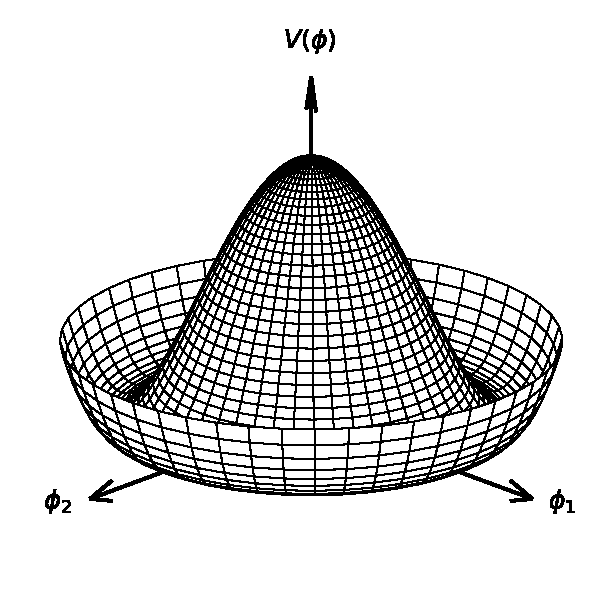
\includegraphics[width=0.5\textwidth]{Figures/standard_model/mexican_hat_potential}
	\caption{The form of the Higg's potential $V(\phi)$ if $\mu^2 < 0$ and $\lambda > 0$ respect to the first component of the complex doublet}
	\label{fig:mexican_hat}
\end{figure}

As shown in \Cref{fig:mexican_hat}, the potential has an infinite number of vacuum states satisfying this condition.
Physically, the vacuum will fall into one of these states, spontaneously breaking the symmetry of the Lagrangian.
With no loss of generality, the physical vacuum state is chosen to be,
\begin{equation}
	\label{eq:higgs_vacuum}
	| 0 \rangle	= \frac{1}{\sqrt{2}} \begin{pmatrix} 0 \\ v \end{pmatrix}.
\end{equation}
In order to use perturbation theory, the field $\phi$ is expanded about the vacuum state $|0\rangle$,
\begin{equation}
	\phi(x) = \frac{1}{\sqrt{2}} \begin{pmatrix} \phi_1(x) + i \phi_2(x) \\ v + \phi_3 + i \phi_4(x) \end{pmatrix}.
\end{equation}

The expected form of the symmetry breaking should result in the group of QED,
\begin{equation}
	\text{SU}(2)_L \times \text{U}(1)_Y \rightarrow_\text{EWSB} \text{U}(1)_\text{Q},
\end{equation}
where $Q$ refers to the electric charge.
The Goldstone theorem states that for every spontaneously broken continuous symmetry, there exists a massless scalar boson; one for each generator of the group.
In EWSB, the broken symmetry should result in three massless Goldstone bosons, however there is no experimental evidence for such massless scalar particles.
The Higgs mechanism resolves this by absorbing the Goldstone bosons through an appropriate selection of gauge.
It's crucial to note that physical predictions remain unchanged regardless of the gauge, but by selecting the \textit{unitary gauge}, the Goldstone bosons vanish, and the fields in the Lagrangian represent the actual physical particles.
In the unitary gauge the scalar field is given by,
\begin{equation}
	\label{eq:higgs_unitary_gauge}
	\phi(x) = \frac{1}{\sqrt{2}} \begin{pmatrix} 0 \\ v + h(x) \end{pmatrix},
\end{equation}
where $h(x)$ is the physical massive Higgs field, the excitation of which is the Higgs boson $H$.

The relationship between weak isospin, hypercharge, and electric charge is given by,
\begin{equation}
	\label{eq:hypercharge}
	Q = I^3 + \frac{Y}{2}.
\end{equation}
As the only surviving massless boson is the photon, $\text{U}(1)_\text{Q}$ must remain a symmetry of the vacuum state.
This is achieved by setting the electric charge of the vacuum state to zero, or equivalently $Y=1$.
Using the definitions from \Cref{eq:pauli_matrices} and \Cref{eq:ew_covariant_derivative} the covariant derivative is given by
\begin{equation}
	\label{eq:higgs_covariant_derivative}
	D_\mu = \frac{1}{2}
	\begin{pmatrix}
		2 \partial_\mu + i g_W W_\mu^3 + i g_Y B_\mu &
		i g_W (W_\mu^1 - i W_\mu^2)                    \\
		i g_W (W_\mu^1 + i W_\mu^2)                  &
		2 \partial_\mu - i g_W W_\mu^3 + i g_Y B_\mu
	\end{pmatrix}
\end{equation}
Combining this with the unitary gauge scalar field yields the first term of the Higgs Lagrangian,
\begin{align}
	\label{eq:higgs_lagrangian_1}
	\begin{split}
		(D_\mu \phi)^\dagger (D^\mu \phi) =
		\frac{1}{2} \partial_\mu h \partial^\mu h
		+ \frac{1}{8} g_W^2 (W_\mu^1 + i W_\mu^2)(W^{1\mu} - i W^{2\mu})(v + h)^2
		\\
		+ \frac{1}{8} (g_W W_\mu^3 - g_Y B_\mu)(g_W W^{3\mu} - g_Y B^\mu)(v + h)^2.
	\end{split}
\end{align}
One can identify the massive physical fields by the terms in \Cref{eq:higgs_lagrangian_1} that are quadratic in the gauge boson fields and do not contain the Higgs field.
\begin{equation}
	W^\pm_\mu = \frac{W^1_\mu \mp i W^2_\mu}{\sqrt{2}}
	\qquad
	Z_\mu = \frac{g_W W^3_\mu - g_Y B_\mu}{\sqrt{g_W^2 + g_Y^2}}
	\qquad
	A_\mu = \frac{g_W B_\mu + g_Y W^3_\mu}{\sqrt{g_W^2 + g_Y^2}}.
\end{equation}
Rewriting out \Cref{eq:higgs_lagrangian} in terms of the physical fields and in the unitary gauge gives,
\begin{equation}
	\label{eq:higgs_lagrangian_full}
	\resizebox{.99\hsize}{!}{$
			\begin{aligned}
				\mathcal{L}_{EW+H}
				 & = \underbrace{\vphantom{\frac{}{}} - \lambda v^2 h^2}_{H \text{ mass}}
				\underbrace{+\frac{1}{4} g_W^2 v^2 W^-_\mu W^{+\mu}}_{W \text{ mass}}
				\underbrace{+\frac{1}{8} g_Y^2 v^2 Z_\mu Z^\mu}_{Z \text{ mass}}                                                                                 \\
				 & \underbrace{+\frac{1}{2} g_W^2 v h W^-_\mu W^{+\mu}}_{HWW}
				\underbrace{+\frac{1}{4} g_W^2 h^2 W^-_\mu W^{+\mu}}_{HHWW}
				\underbrace{+\frac{1}{4} g_Y^2 v h Z_\mu Z^\mu}_{HZZ}
				\underbrace{+\frac{1}{8} g_Y^2 h^2 Z_\mu Z^\mu}_{HHZZ}                                                                                           \\
				 & \underbrace{+\frac{1}{2}(\partial_{\mu} h)(\partial^{\mu} h) - \lambda v h^3 + \frac{1}{4}\lambda h^4}_{h\text{ dynamics and self-couplings}}
				\underbrace{+\frac{1}{4} W^a_{\mu\nu} W^{a,\mu\nu} + \frac{1}{4} B_{\mu\nu} B^{\mu\nu}}_{\text{EW dynamics and self-couplings}}.
			\end{aligned}
		$}
\end{equation}
From the top row of \Cref{eq:higgs_lagrangian_full} the masses of each of the bosons can be identified,
\begin{equation}
	\label{eq:ew_masses}
	m_W = \frac{1}{2} g_W v
	\qquad
	m_Z = \frac{1}{2} v \sqrt{g_W^2 + g_Y^2}
	\qquad
	m_A = 0
	\quad
	m_H = \sqrt{2 \lambda} v.
\end{equation}
The bottom row of \Cref{eq:higgs_lagrangian_full} includes the dynamics and self-couplings of the electroweak fields in their original form before EWSB due to convenience.
Expanding this term with respect to the physical fields results in trilinear interactions between the photon and the $W^\pm$ bosons.
The free parameters of the GSW + Higgs mechanism are the electroweak coupling constants $g_W$ and $g_Y$, the Higgs self-coupling $\lambda$, and the vacuum expectation value $v$, all of which are determined experimentally.

The final piece of the SM is the generation of fermion masses through the Higgs mechanism.
Due to the different transformation properties of the left- and right-handed fermions, the standard mass term $m \bar \psi \psi$ mixes the left- and right-handed components and thus is not invariant under the electroweak symmetry group.
The Yukawa interaction term is introduced to couple each of the fermions doublets to the Higgs field.
For example the electron mass term is given by,
\begin{equation}
	\label{eq:yukawa}
	\begin{split}
		\mathcal{L}_\text{Yukawa} & = -g_e( \bar \psi_L \phi \psi_R + \bar \psi_R \phi^\dagger \psi_L)    \\
		                          & = -g_e \left[
			\begin{pmatrix} \bar \nu_e & \bar e \end{pmatrix}_L \begin{pmatrix} 0 \\ \frac{v + h}{\sqrt{2}} \end{pmatrix} e_R
			+ \bar e_R \begin{pmatrix} 0 & \frac{v + h}{\sqrt{2}} \end{pmatrix} \begin{pmatrix} \nu_e \\ e \end{pmatrix}_L
		\right]                                                                                           \\
		                          & = -\frac{g_e v}{\sqrt{2}} \bar e e - \frac{g_e}{\sqrt{2}} \bar e e h,
	\end{split}
\end{equation}
where $g_e$ is the electron Yukawa coupling constant.
A similar prescription can be applied other leptons, the up-type, and down-type quarks to yield the relationship of the fermion masses $m_f$ to the Yukawa coupling constants $g_f$ and the Higgs vacuum expectation value,
\begin{equation}
	\label{eq:fermion_mass}
	m_f = \frac{g_f v}{\sqrt{2}}.
\end{equation}

\section{Particle Jets}
\label{sec:jets}

In particle physics, jets are collimated streams of particles moving together in a cone-like structure that typically was initiated by a high-energy quark or gluon.
A common feature in high-energy collisions, jets are emergent phenomena that arise due to the nature of QCD.
Simply put, if a high-energy quark or gluon is emitted from a collision, it quickly radiates gluons which in turn either radiate more gluons or which split into quark-antiquark pairs.
This continues until the energy of the particles is low enough that they form stable colour-neutral bound states.
Jets are therefore formed during the transition from the perturbative to the non-perturbative regimes of QCD.

Jet formation can be highlighted by the Feynman diagram in \Cref{fig:quark_gluon}.
Here a quark propagator, produced in some inelastic collision, radiates a gluon.
This specific diagram becomes dominant when the virtual propagator is close to being on-shell.
This condition is satisfied in two limits which are essential in jet physics.
One is referred to as the \textit{collinear limit} where the angle between the quark and the gluon approaches zero.
This indicates preference for collinear radiation and explains why jets are collimated in the direction of the initiating particle\footnote{Jets are also collimated when measured in the lab frame due to the large boost of the initiating particle.}.
The other is the \textit{soft limit} where the energy of the gluon approaches zero.
Practically, this means that each time a parton is emitted, it is accompanied by a soft haze of radiation.
These conditions exist for all gauge theories, but are particularly important for QCD due the strength of $\alpha_s$ even at high energies.

\begin{figure}[h]
	\centering
	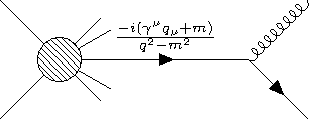
\includegraphics[width=0.5\textwidth]{Feynman/quark_gluon.pdf}
	\caption{Simple diagram of a quark emitted from some collision radiating a gluon. The matrix element of this process has a singularity when the virtual propagator is close to being on-shell ($q^2\approx m^2$) which is satisfied in the collinear and soft limits.}
	\label{fig:quark_gluon}
\end{figure}

Another view of jet formation is through the process of breaking colour strings between quarks.
From confinement, if two quarks were produced back-to-back in a collision, the color field between them would be squeezed into a color string with constant energy density.
As they move apart, it becomes energetically favourable to create a quark-antiquark pair from the vacuum, leading to two new strings.
If the quarks were produced with enough energy, this process repeats until the energy is low enough that the stable colour-neutral bound states emerge as shown by \Cref{fig:hadronisation}.
Where exactly the strings break is ambiguous, resulting in the highly stochastic nature of jets.
The lightest hadrons are the most accessible to this process, which is why typically jets are composed primarily of pions ($\approx80\%$) and kaons ($\approx15\%$).

\begin{figure}[h]
	\centering
	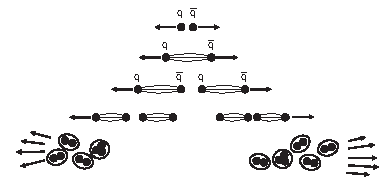
\includegraphics[width=0.8\textwidth]{Figures/standard_model/hadronisation.pdf}
	\caption{Qualitative picture of the formation of two jets via the splitting of color flux-tubes causing hadronisation \cite{ModernParticlePhysics}.}
	\label{fig:hadronisation}
\end{figure}

While jets are essentially sets or clusters of many particles, they can also be defined by their own kinematics, calculated by summing up the four-momenta of all of its constituents.
Furthermore, even if the original parton was massless, the jet as a whole may have non-zero invariant mass due to noncollinear radiation.
The nature and shape of this radiation is characteristic of the properties of the initiating parton.
This point is crucial for understanding jet physics and defining jet algorithms which is discussed in \Cref{sec:jets_reconstruction}.

\section{Standard Model Limitations and Open Questions}
\label{sec:sm_limitations}

Predictions made by the SM have been confirmed to an extraordinary degree of precision in collider experiments, as shown by \Cref{fig:sm_precision}.
Despite this, there are several reasons to believe that the SM is not the final theory of particle physics.
Many perceived shortcomings of the SM lead to open questions that define the regions of active research in particle physics as well as many proposed extensions to the SM\@.

For example, gravity is a notable omission from the SM owing to the lack of a renormalizable QFT for gravity.
Candidate theories for a quantum theory of gravity include string theory and loop quantum gravity~\cite{GravityQFT}.
However, gravity is so weak that it is unlikely a theory of quantized gravity could even make testable predictions at the energies accessible by current experiments.

\begin{figure}
	\centering
	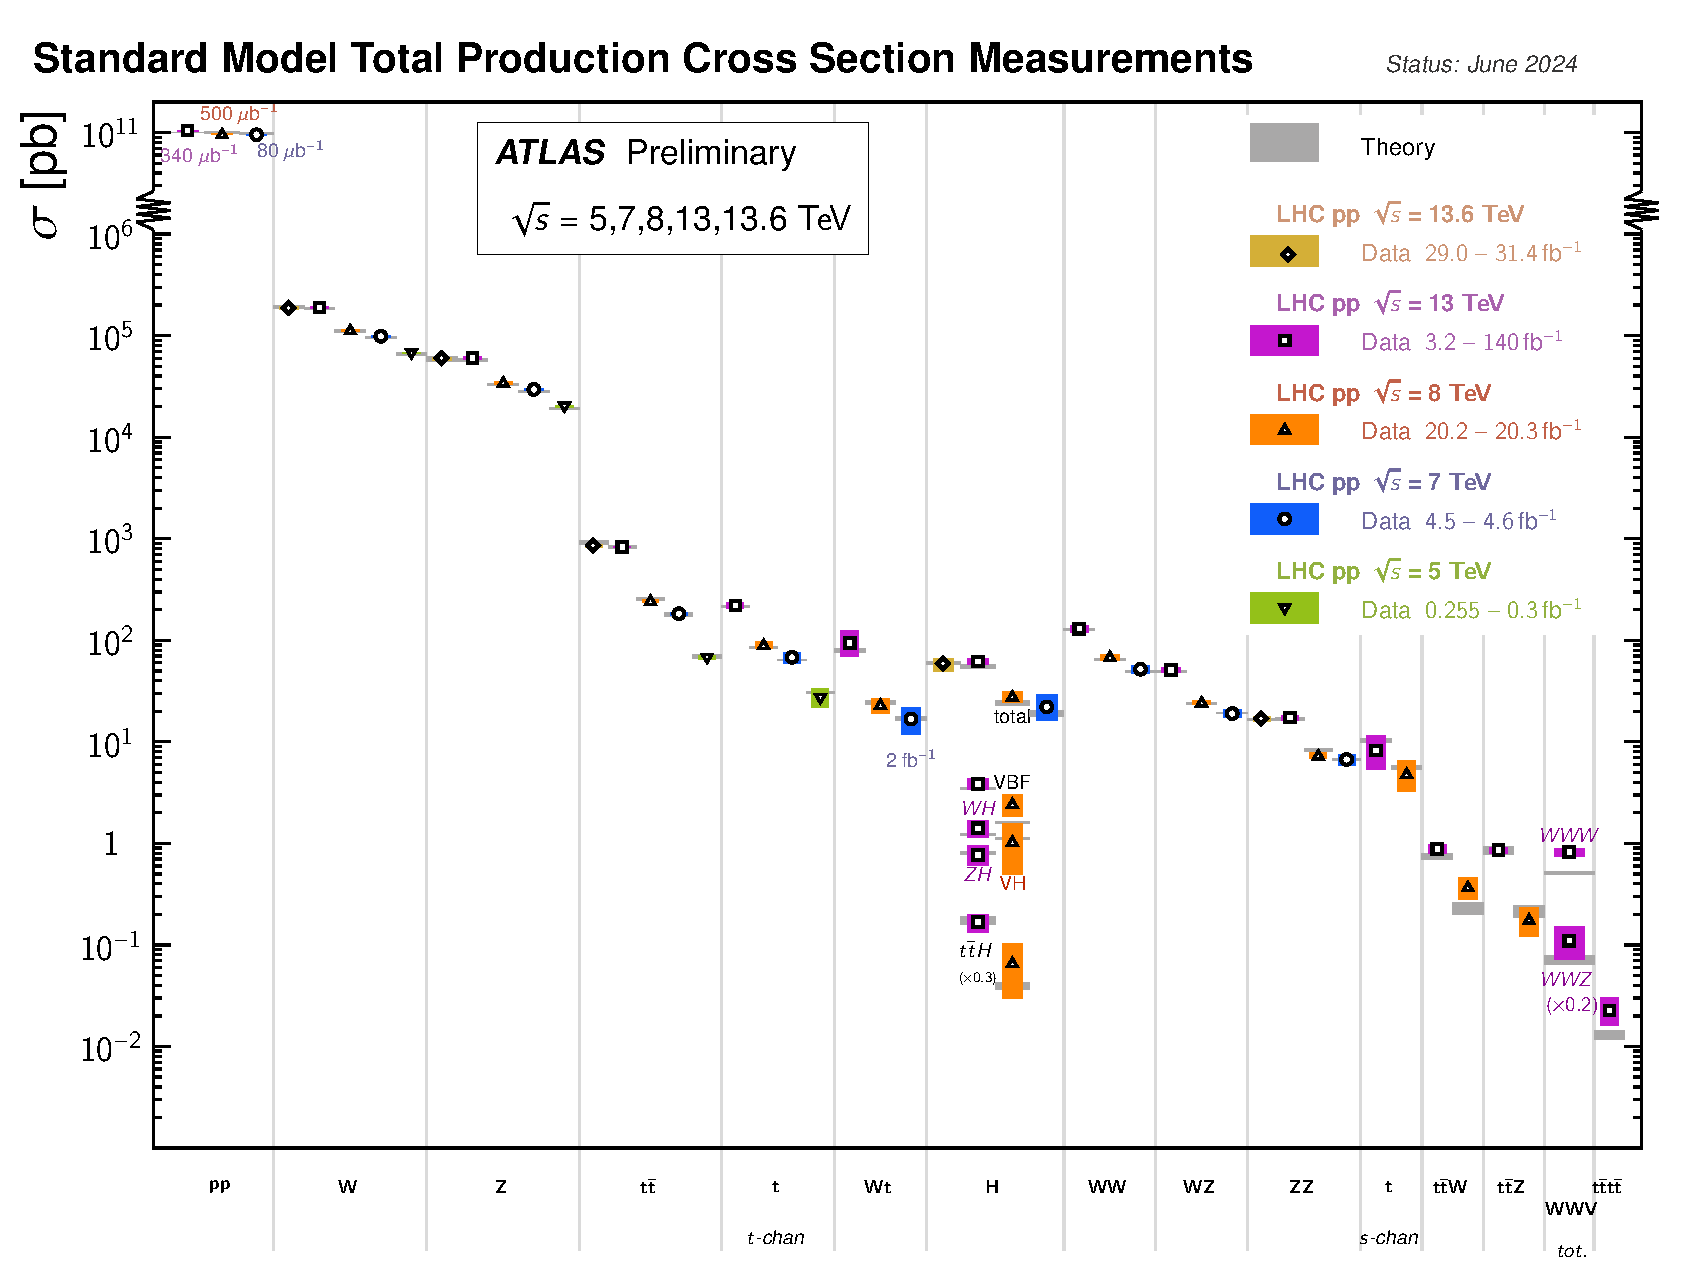
\includegraphics[width=0.7\textwidth]{Figures/standard_model/sm_summary.pdf}
	\caption{Comparison of the total production cross-sections of various processes predicted by the SM and measured by the ATLAS experiment \cite{ATLAS:2024cgh}.}
	\label{fig:sm_precision}
\end{figure}

Cosmological observations dating back to the 1930s~\cite{GalaxyRotation} have shown that the majority of the gravitational effects in the universe is not a result of visible matter.
This was first observed by the movements of galaxies within clusters~\cite{GalaxyRotation}, but has since been independently supported by measurements of the rotation of galaxies themselves~\cite{DistributionDarkMatter, EvidenceDarkMatter,NumericalStudyStability}, gravitational lensing~\cite{GravitationalLensMagnification, Lensing1, Lensing2},
hot gas in galaxy clusters~\cite{HotGas}, and the cosmic microwave background~\cite{Planck2018Results}.
The current theory to explain these phenomena is the presence of cold dark matter (CDM) which accounts for 85\% of the mass content in the universe~\cite{Planck2018Results}.
In this model CDM particles that must be stable, massive, and at most weakly interacting, and there is no candidate in the SM that fits this description.
Furthermore, inthe current model cosmology, $\Lambda$CDM, the dominant energy in the universe is \textit{dark energy}~\cite{LCDM1, LCDM2, LCDM3, LCDM4} a positive pressure of the vacuum that is causing the universe to expand at an accelerating rate for which there is no explanation in the SM\@.

In the SM, anti-matter is treated as a mirror image of matter, however the universe is almost entirely composed of matter \cite{AlexDM1, AlexDM2}
There exist two possibilities for this discrepancy; either the universe began with a preference for matter over anti-matter, or the universe was initially symmetric, and some process called \textit{baryogenesis}~\cite{BaryosynthesisOriginGalaxies}, occurred to create the imbalance.
While there is no clear evidence for either scenario, the latter is more appealing to many physicists.
The Sakharov conditions~\cite{Sakharov1967} for baryogenesis are that it violates baryon number, C and CP symmetry, and must have occured before the universe reached thermal equilibrium.
CP violation is present in the SM from the CKM and PMNS matrices, but it is not sufficient to explain the observed matter-antimatter asymmetry.
It is hoped that there exist new physical processes beyond the SM that induces the much larger CP violation required for baryogenesis.

The above issues are related with the SM's inability to describe cosmological phenomena.
An additional set of ``issues'' are derived from asthetic or philosophical considerations.
The SM has 19 free parameters that must be determined experimentally, a value considered by many to be too large to be considered a fundamental theory.
Another issue is the \textit{hierarchy problem}.
In a QFT, physical observables are determined by the sum of all possible Feynman diagrams, which often includes divergent terms.
These divergences are removed by renormalization which fixes the parameters of the theory to the observed values.
However, in the case of the Higgs mass, the one-loop corrections are around 16 orders of magnitude larger than the observed value.
To resolve this, the bare mass of the Higgs must be fine-tuned to an accuracy of 1 part in $10^{16}$, which many physicists find unsatisfactory.
Finally, the unification of QED and the weak force led many to develop Grand Unified Theories (GUTs)~\cite{GUT1, GUT2} which predict that all forces in the SM are unified at high energies.
Many of the predictions of GUTs, such as proton decay, have not been observed, and the energy scale at which the forces unify is far beyond the reach of current experiments.
